\subsection{Bijlage 2: Berekening rolweerstand}

\subsubsection{De rolweerstand op Aarde}

Een belangrijke eigenschap van de Rover is de rolweerstand. Dit heeft een grote invloed in de effici\"entie van het rijden. Met een grote rolweerstand komt de wagen veel sneller tot stilstand dan bij een kleine rolweerstand. Het bepalen van de rolweerstand is niet moeilijk. Met behulp van een schuine plank is het mogelijk het verband te zoeken tussen de hoogte van waarop de wagen is losgelaten en de afstand die de wagen heeft afgelegd nadat het van de plank reed.\\
Wanneer de wagen boven op de plank staat, heeft het door de zwaartekracht een zekere potenti\"ele energie.

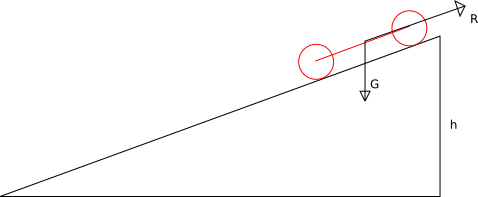
\includegraphics[width=10cm]{bijlagen/bijlage-2/rolweerstand.png}

\begin{equation}
E_{pot}=m*g*h
\end{equation}
Wanneer de wagen naar beneden rolt, zet het die potenti\"ele energie om in kinetische energie.
\begin{equation}
E_{kin}=\frac{m*v^2}{2}
\end{equation}
Aan de onderkant van de helling is alles omgezet in kinetische energie. De snelheid $v$ is nu te berekenen door de vorige 2 formules aan elkaar gelijk te stellen. Voor het berekenen van deze snelheid wordt de wrijving met de grond tijdens het rijden op de helling verwaarloosd. Dit is echter een redelijke veronderstelling doordat de wrijving zeer klein is ten opzichte van de zwaartekracht.\\
Terwijl de wagen verder rolt, verliest het deze energie door de wrijving met de grond. Uit de bewegingsvergelijking hieronder kan de versnelling $a$ berekend worden.
\footnote{Deze vergelijking werd afgeleid door team 208 in P\&O opdracht 3}
\begin{equation}
x=\frac{1}{2}*\left(\frac{-v}{a}\right)^2+v*\left(\frac{-v}{a}\right)
\end{equation}
Terwijl de wagen verder rolt, spelen er drie krachten op in. Dit zijn de zwaartekracht, de normaalkracht en de wrijvingskracht. Aangezien de wagen horizontaal rijdt, heeft alleen de wrijvingskracht invloed op de versnelling. Met behulp van het $2\textsuperscript{de}$ Postulaat van Newton kan de rolweerstand bepaald worden.
\begin{equation}
F_{rol}=F_{res}=m*a
\end{equation}
Ten slotte wordt de wrijvingsco\"effici\"ent $\mu$ bepaald met behulp van de definitie van de rolweerstand.
\begin{equation}
\mu=\frac{F_{rol}}{F_{normaal}}=\frac{F_{rol}}{m*g}
\end{equation}
%Dit moet aangepast worden
%geen "worden" en verleden tijd
Om de onnauwkeurigheid van meetresultaten zo goed mogelijk te beperken, werd dit experiment zes keren herhaald. De definitieve wrijvingscoëffici\"ent is het gemiddelde van de zes bekomen coëfficiënten. deze waarde bedraagt:$$\mu=0.067$$
\pagebreak
\subsubsection{De rolweerstand op Mars}
Het vinden van de rolweerstand op Mars gebeurt op een zeer gelijkaardige manier als het vinden van de rolweerstand op Aarde. Het enige verschil is de gravitatieconstante $g$. Om de gravitatieconstante van Mars te berekenen, bestaat de volgende formule.
\begin{equation}
g=\frac{G*m_{Mars}}{\left(r_{Mars}\right)^2}
\end{equation}
Wanneer deze nieuwe gravitatieconstante ingevuld wordt in de vorige vergelijkingen, wordt de nieuwe rolweerstand $$F_{rol}=0.12N$$